\documentclass[12pt]{article}
\usepackage{german}
\usepackage{todonotes}
\usepackage{tikz}
\usepackage[utf8]{inputenc}
\usepackage{adjustbox}
\usepackage{graphicx}
\usepackage{afterpage}
\usepackage{float}
\graphicspath{{./images/}}

\begin{document}

%\listoftodos
\tableofcontents
\newpage

\part{Erianet}
\section{Einleitung}
%\todo{Namensherkunft}
\paragraph{}
Das Erianet ist eine mit Python entwickelte Software, die
durch ein Neurales Netzwerk f"ahig ist,
Personen anhand ihrer Gesichter unterscheiden.
Es wurde von Mayrhofer Erik und Schwarcz Florian
entwickelt und durch Kombination beider Vornamen und \glqq neural net\grqq{}
auf seinen Namen getauft.
%\todo{Warum Projekt?}
\paragraph{}
Im Rahmen des Schulunterrichts im Fach \glqq Systemplanung und Projektentwicklung\grqq{}
war es die Aufgabe des Projektteams, eine zur Gesichtserkennung
f"ahige Software zu entwickeln.
%\todo{Welche Technologien}
Bei der Entwicklung bediente man sich einiger Python-Libraries.
So wurde OpenCV als Gesichtsdetektor eingesetzt und mit Keras das neurale
Netz erstellt und trainiert.
\paragraph{}
Zum Trainieren des Modells wurden vorgefertigte Sammlungen f"ur genau diesen
Zweck auf dem Internet verwendet. Einige davon waren die \glqq Labelled Faces in the Wild\grqq{},
\glqq AT\&T Faces\grqq{} und \glqq YouTube face database\grqq{}. Es wurden
auch selbst Bilder mit einem dazu erstellten Programm geschossen und zum Training verwendet.
\section{Architektur}
\newpage
\afterpage{\clearpage}
\begin{figure}[H]
    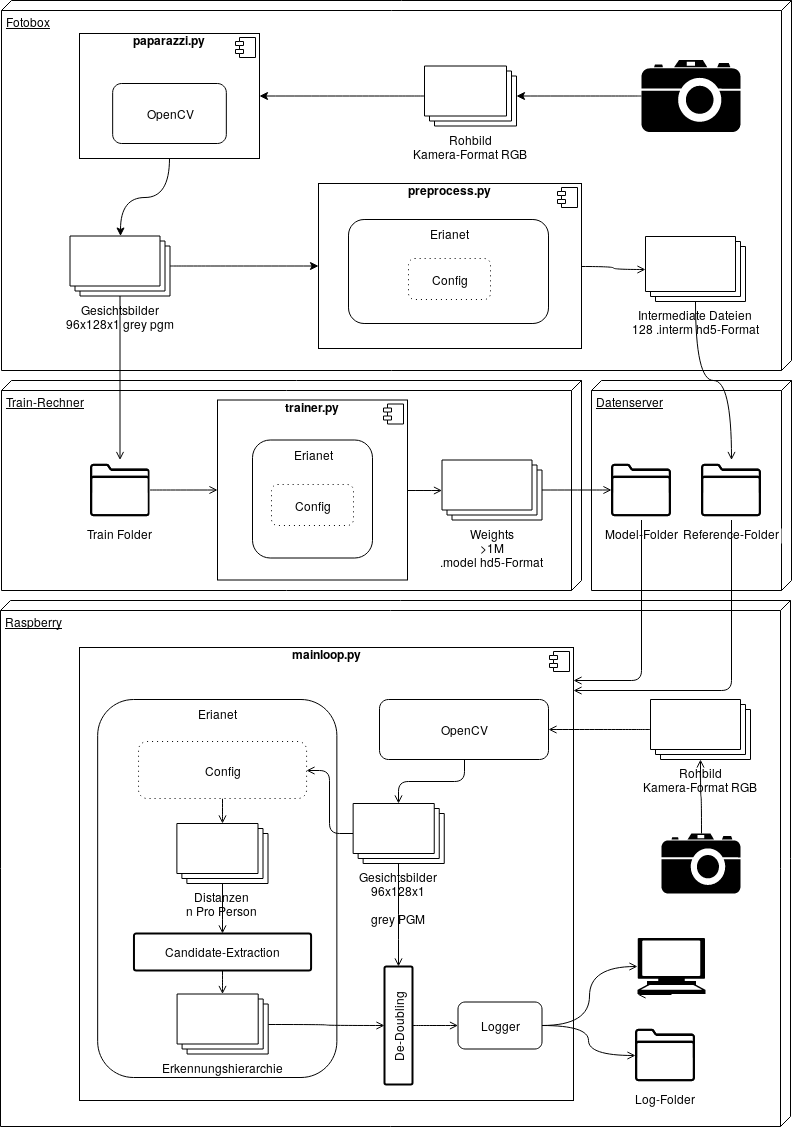
\includegraphics[height=0.9\textheight]{Architektur}
    \caption{Architektur}
\end{figure}

\subsection{Fotobox}
Die Fotobox ist ein kleiner Rechner,
mit dessen Hilfe Referenzbilder aufgenommen werden
k"onnen.
\paragraph{paparazzi.py}
greift den Kamera-Feed einer Webcam ab, und nutzt
OpenCVs Haar-Classifier dazu ein erkanntes Gesicht 
herauszuschneiden. Dieses wird dann in unser verwendetes
Format (\ref{formats}).
\paragraph{preprozess.py}
nimmt die, vorher aufgenommenen Bilder und 
\subsection{Train-Rechner}
\subsection{Raspberry}
\subsection{Formate}
\label{formats}

%\todo{Diagramm mit Annotationen}
%\todo{Kapitel f"ur alle Annotationen}
\section{Neurales Netz}
%\todo{Erweiterung zu Kaptiel in Architektur}


\part{Facepong}
\section{Einleitung}
%\todo{Was Warum und Spielweise}
\paragraph{}
F"ur den Tag der offenen T"ur an der HTL Leonding wurde dem Projektteam
aufgetragen, mithilfe ihrer gesammelten Erfahrung im Bereich Gesichtsdetektion
ein kleines Programm zu entwickeln, welches man den Besuchern Vorstellen kann.
Dabei kam die Idee auf, ein Spiel zu programmieren, bei dem man mit seinem Gesicht
gegen einen anderen Spieler das klassische Spiel \glqq Pong\grqq{} spielen kann.
\paragraph{}
Zus"atzlich zu OpenCV f"ur die Gesichtsdetektion wurde in diesem Teil des Projektes
die Library PyGame f"ur realistische Physiksimulation und einfache Bildausgabe
herangezogen.
\section{Aufbau und Spielweise}
\paragraph{}
Zum Spielen braucht man eine Kamera und einen Monitor bzw. Beamer. Die Kamera
wird m"oglichst mittig entweder unter oder "uber der Bildausgabe aufgestellt und angeschlossen.
Anschließend wird das Programm gestartet und es kann gespielt werden.
Betreten die beiden Spieler ihren Bereich links und rechts vor der Kamera,
startet das Spiel automatisch. Der Ball kann nun mit dem Kopf angestoßen werden
und muss das Tor des Gegners ber"uhren. Zu beachten ist hierbei, dass
das Gesicht jederzeit gerade zur Kamera gerichtet sein muss, damit es erkannt werden kann.
\section{Probleme und Zukunftspl"ane}
\paragraph{}
%\todo{Probleme und Z.}
Wie bereits erw"ahnt muss man den Kopf zu jeder Zeit gerade in Richtung
der Kamera halten. Dadurch wird bei zu großer Neigung durch nach unten oder zur
Seite blicken das Spiel angehalten, da kein Gesicht erkannt wird.
\paragraph{}
Zuk"unftige Verbesserungen w"aren zum einen die Behebung des oben genannten Problems
durch Einsatz besserer Modelle unter Beachtung der Performance. Das Spiel l"auft aktuell
in 480p und verlangsamt sich beim Upgrade auf 1080p auf unter 10 Bilder pro Sekunde,
was auf das inperformante Modell zur Gesichtsdetektion zur"uckzuf"uhren ist.
F"ur den jetzigen Einsatz mit Beamer und Kamera sind 480p jedoch ausreichend.
\section{Architektur}
%\todo{Architektur}
\end{document}